\chapter{Les axiomes de l'origami}\label{c.origami-axioms}

%%%%%%%%%%%%%%%%%%%%%%%%%%%%%%%%%%%%%%%%%%%%%%%%%%%%%%%%%%%%%%%



%%%%%%%%%%%%%%%%%%%%%%%%%%%%%%%%%%%%%%%%%%%%%%%%%%%%%%%%%%%%%%%

L'origami, l'art du pliage du papier, a été développé il y a plusieurs siècles au Japon et connaît aujourd'hui un succès mondial. La théorie mathématique de l'origami a été développée à la fin du \textsc{xx}$^\text{e}$ siècle. Elle repose sur un ensemble de sept axiomes, les \og axiomes de  Huzita-Hatori\fg{}, du nom de Humiaki Huzita qui a formalisé les six premiers axiomes et de Koshiro Hatori qui a trouvé le septième. Jacques Justin a publié les sept axiomes plusieurs années avant Huzita et Hatori, et Margherita P. Beloch a formulé le sixième axiome en 1936. Néanmoins, les axiomes sont connus comme les axiomes de Huzita-Hatori\footnote{N.D.T. \og Axiomes de Justin-Huzita-Hatori\fg{} dans \cite{Delahaye}.} .

Dans une suite de trois chapitres, nous allons explorer les mathématiques de l'origami. Ce chapitre présente les axiomes, le chapitre~\ref{c.origami-cube} relie l'origami aux racines des polynômes et le chapitre~\ref{c.origami-constructions} montre que les constructions avec l'origami peuvent résoudre des problèmes impossibles à résoudre à la règle et au compas.
 
Ce chapitre contient une section pour chacun des sept axiomes. Après l'énoncé d'un axiome et un diagramme du pli qu'il spécifie, on présente les équations du pli et des points d'intersection en utilisant la géométrie analytique. Un pli peut également être défini comme un lieu géométrique, c'est-à-dire l'ensemble de tous les points satisfaisant à une certaine propriété. Le terme \og pli\fg{} vient de l'opération d'origami consistant à plier une feuille de papier, mais il est utilisé ici pour désigner la droite qui serait créée par le pliage du papier.

Les plis se traduisent par des réflexions. Étant donné un point $p$, son symétrique par rapport au pli $l$ est un point $p'$ tel que $l$ soit la médiatrice du segment  $\overline{pp'}$  (fig.~\ref{f.origami-def}).

\begin{figure}[h]
\centering
\begin{tikzpicture}[scale=.8]
\coordinate (P1) at (2,2);
\coordinate (P1P) at (6,4);
\coordinate (mid) at (4,3);
\draw[rotate=30] (mid) rectangle +(8pt,8pt);
\coordinate (m1) at ($(P1)!.5!(mid)$);
\coordinate (m2) at ($(mid)!.5!(P1P)$);
\draw[thick] (m1) -- +(120:4pt);
\draw[thick] (m1) -- +(-60:4pt);
\draw[thick] (m2) -- +(120:4pt);
\draw[thick] (m2) -- +(-60:4pt);
\draw[thick] (P1) -- (P1P);
\draw[very thick,dashed] (4.7,1.6) -- node[very near end,right,yshift=4pt] {$l$} (3.5,4);
\vertex{P1};
\vertex{P1P};
\node[above left] at (P1) {$p$};
\node[above left] at (P1P) {$p'$};
\draw[very thick,dotted,->,bend right=50] (2.1,1.9) to (6.05,3.9);
\end{tikzpicture}
%\includegraphics[width=0.4\textwidth]{Fig10_1}
\caption{Le pli est la médiatrice du segment qui relie un point et son image.}\label{f.origami-def}
\end{figure}


\section{Axiome 1}\label{s.ax1}


\begin{axiom}
Etant donné deux points distincts $p_1=(x_1,y_1)$ et  $p_2=(x_2,y_2)$, il existe un pli unique $l$ qui passe par ces deux points (fig.~\ref{f.origami-axiom1}).
\end{axiom}



\noindent\textbf{Détermination de l'équation du pli.}
L'équation du pli $l$ se déduit des coordonnées de $p_1$ et $p_2$. La pente est le quotient des différences des coordonnées:
\begin{align}
y - y_1 = \frac{y_2-y_1}{x_2-x_1}(x-x_1)\,.
\end{align}

\begin{figure}[bhtp]
\centering
\begin{tikzpicture}[scale=0.9]
\draw[step=10mm,white!50!black,thin] (-1,-1) grid (8,6);
\draw[thick] (-1,0) -- (8,0);
\draw[thick] (0,-1) -- (0,6);
\foreach \x in {0,...,8}
  \node at (\x-.2,-.2) {\sm{\x}};
\foreach \y in {1,...,6}
  \node at (-.2,\y-.3) {\sm{\y}};
\coordinate (P1) at (2,2);
\coordinate (P2) at (6,4);
\draw[very thick,dashed] ($(P1)!-.75!(P2)$) -- node[very near end,below] {$l$} ($(P1)!1.5!(P2)$);
\vertex{P1};
\vertex{P2};
\node[above left] at (P1) {$p_1$};
\node[above left] at (P2) {$p_2$};

\draw[very thick,dotted,->,bend left=30] (2,5) to (4,1);
\end{tikzpicture}
%\includegraphics[width=0.8\textwidth]{Fig10_2}
\caption{Axiome  $1$.}\label{f.origami-axiom1}
\end{figure}

\begin{example}
Soient  $p_1=(2,2)$ et $p_2=(6,4)$. L'équation de $l$ est 
\begin{align*}
y-2&=\frac{4-2}{6-2}(x-2)\,,\\
y&=\frac{1}{2}x+1\,.
\end{align*}
\end{example}

%%%%%%%%%%%%%%%%%%%%%%%%%%%%%%%%%%%%%%%%%%%%%%%%%%%%%%%%%%%%%%%%


\section{Axiome 2}\label{s.ax2}



\begin{axiom}
Étant donné deux points distincts $p_1=(x_1,y_1)$ et  $p_2=(x_2,y_2)$, il existe un pli unique $l$ qui place $p_1$ sur $p_2$ (fig.~\ref{f.origami-axiom2}).
\end{axiom}

Le pli est le lieu géométrique de tous les points équidistants de $p_1$ et $p_2$.\\

\begin{figure}[ht]
\centering
\begin{tikzpicture}[scale=1]
\draw[step=10mm,white!50!black,thin] (-1,-1) grid (8,6);
\draw[thick] (-1,0) -- (8,0);
\draw[thick] (0,-1) -- (0,6);
\foreach \x in {0,...,8}
  \node at (\x-.2,-.2) {\sm{\x}};
\foreach \y in {1,...,6}
  \node at (-.2,\y-.3) {\sm{\y}};
\coordinate (P1) at (2,2);
\coordinate (P2) at (6,4);
\coordinate (mid1) at ($(P1)!.5!(P2)$);
\coordinate (mid2) at ($(P1)!.5!(P2)+(-1,2)$);

\draw[rotate=30] (mid1) rectangle +(8pt,8pt);

\draw (P1) -- (P2);
\draw[very thick,dashed] ($(mid1)!-1.4!(mid2)$) -- node[very near end,left,yshift=-12pt] {$l$} ($(mid1)!1.4!(mid2)$);
\vertex{P1};
\vertex{P2};
\node[above left] at (P1) {$p_1$};
\node[above left] at (P2) {$p_2$};

\draw[very thick,dotted,->,bend right=50] (2.1,1.9) to (6,3.9);
\end{tikzpicture}
%\includegraphics[width=0.9\textwidth]{Fig10_3}
\caption{Axiome  $2$.}\label{f.origami-axiom2}
\end{figure}

\noindent\textbf{Détermination de l'équation du pli.}
Le pli $l$ est la médiatrice de $\overline{p_1p_2}$. Sa pente est l'inverse de l'opposé de la pente de la droite qui relie $p_1$ et $p_2$. Le pli $l$ passe par le milieu des deux points :
\begin{align}
y - \frac{y_1+y_2}{2} = -\frac{x_2-x_1}{y_2-y_1}\left(x-\frac{x_1+x_2}{2}\right)\,.\label{eq.midpoint1}
\end{align}

\begin{example}
Soient $p_1=(2,2)$ et $p_2=(6,4)$. L'équation de $l$ est 
\begin{align*}
y-\left(\frac{2+4}{2}\right)&=-\frac{6-2}{4-2}\left(x-\left(\frac{2+6}{2}\right)\right)\,,\\
y&=-2x+11\,.
\end{align*}
\end{example}

%%%%%%%%%%%%%%%%%%%%%%%%%%%%%%%%%%%%%%%%%%%%%%%%%%%%%%%%%%%%%%%%


\section{Axiome 3}\label{s.ax3}


\begin{axiom}
Étant donné deux droites $l_1$ et $l_2$, il existe un pli $l$ qui place $l_1$ sur $l_2$. (fig.~\ref{f.origami-axiom3}).
\end{axiom}

Le pli est le lieu géométrique des points qui sont équidistants de $l_1$ et $l_2$, où la distance d'un point à une droite est la longueur du segment passant par le point et perpendiculaire à la droite. En utilisant des triangles isométriques, il est facile de montrer que le pli est une bissectrice de l'angle formé par $l_1$ et $l_2$.

\begin{figure}[htbp]
\centering
\begin{tikzpicture}[scale=1]
\draw[step=10mm,white!50!black,thin] (-1,-1) grid (8,7);
\draw[thick] (-1,0) -- (8,0);
\draw[thick] (0,-1) -- (0,7);
\foreach \x in {0,...,8}
  \node at (\x-.2,-.2) {\sm{\x}};
\foreach \y in {1,...,7}
  \node at (-.2,\y-.3) {\sm{\y}};
\coordinate (L1a) at (2,2);
\coordinate (L1b) at (4,6);
\draw (L1a) -- node[very near start,right,yshift=-4pt] {$l_1$} (L1b);
\draw[name path=l1] ($(L1a)!-.75!(L1b)$) -- ($(L1a)!1.25!(L1b)$);
\coordinate (L2a) at (7,1);
\coordinate (L2b) at (4,4);
\draw (L2a) -- (L2b);
\draw[name path=l2] ($(L2a)!-.3!(L2b)$) -- node[very near start,above,xshift=4pt,yshift=2pt] {$l_2$} ($(L2a)!2!(L2b)$);
\path [name intersections = {of = l1 and l2, by = {PM}}];
\node[below left,xshift=-9pt,yshift=-7pt] at (PM) {$p_i$};

\node[above right,xshift=10pt,yshift=4pt] at (PM) {$\alpha$};
\node[below right,xshift=10pt] at (PM) {$\alpha$};
\node[above left,xshift=-3pt,yshift=12pt] at (PM) {$\beta$};
\node[above right,xshift=-3pt,yshift=12pt] at (PM) {$\beta$};

\coordinate (B1a) at (0,4.13);
\coordinate (B1b) at (6,5.1);
\draw[very thick,dashed] ($(B1a)!-.15!(B1b)$) -- node[very near start,above] {$l_{p_1}$}  ($(B1a)!1.35!(B1b)$);

\coordinate (B2a) at (3,6.73);
\coordinate (B2b) at (4,.57);
\draw[very thick,dashed] ($(B2a)!-.05!(B2b)$) -- node[very near end,right,xshift=4pt,yshift=6pt] {$l_{p_2}$} ($(B2a)!1.25!(B2b)$);

\draw[very thick,dotted,->,bend right=50] (6,2.2) to (4.5,6.7);
\draw[very thick,dotted,->,bend left=50] (6.2,1.6) to (1.8,1.3);
\end{tikzpicture}
%\includegraphics[width=0.9\textwidth]{Fig10_4}
\caption{Axiome  $3$.}\label{f.origami-axiom3}
\end{figure}

\noindent\textbf{Détermination de l'équation du pli}

\noindent\textit{$l_1$ et $l_2$ sont parallèles.} Soient $l_1$ d'équation $y=mx+b_1$ et  $l_2$ d'équation $y=mx+b_2$. Le pli est la droite parallèle à $l_1$ et $l_2$ qui est à mi-chemin entre elles :
\[
y=mx+\frac{b_1+b_2}{2}\,.
\]
\noindent\textit{$l_1$ et $l_2$ se croisent.} Soient $l_1$ d'équation  $y=m_1x+b_1$ et  $l_2$ d'équation $y=m_2x+b_2$. Le point d'intersection des deux droites, $p_i=(x_i,y_i)$,  vérifie
\begin{align*}
m_1x_i+b_1&=m_2x_i+b_2\,,\\
x_i &= \frac{b_2-b_1}{m_1-m_2}\,,\\
y_i &=m_1x_i+b_1\,.
\end{align*}

\begin{example}\label{ex.axiom3}
Soient $l_1$ d'équation $y=2x-2$ et $l_2$ d'équation $y=-x+8$. Alors $p_i=(x_i,y_i)$ est donné par
\begin{align*}
x_i&=\frac{8-(-2)}{2-(-1)}=\frac{10}{3}\approx \mbox{3,33}\,,\\
y_i &= 2\cdot\frac{10}{3}-2=\frac{14}{3}\approx \mbox{4,67}\,.
\end{align*}
\end{example}


Le pli est la bissectrice de l'angle formé par $l_1$ et $l_2$ à leur point d'intersection. Il y a deux plis possibles puisqu'il y a deux paires d'angles. Nous devons déterminer les pentes des bissectrices des angles. Si l'angle de la droite $l_1$ par rapport à l'axe $x$ est $\theta_1$ et l'angle de la droite $l_2$ par rapport à l'axe $x$ est $\theta_2$, alors le pli est la droite qui fait un angle  $\theta_b=(\theta_1+\theta_2)/2$ par rapport à l'axe~$x$.

Soient $m_1=\tan\theta_1$ et $m_2=\tan \theta_2$. D'après le théorème~\ref{thm.tangent-sum},  la pente $m_s$ de la droite qui fait un angle  $\theta_1+\theta_2$ avec l'axe $x$ est 
\[
m_s=\tan(\theta_1+\theta_2)= \frac{\tan\theta_1+\tan\theta_2}{1-\tan\theta_1\tan\theta_2}=\frac{m_1+m_2}{1-m_1m_2}\,.
\]
D'après le théorème~\ref{thm.tangent-half},  la pente $m_b$ de la bissectrice de l'angle est 
\[
m_b= \tan\frac{\theta_1+\theta_2}{2}=\frac{-1\pm\sqrt{1+\tan^2(\theta_1+\theta_2)}}{\tan (\theta_1+\theta_2)}=\frac{-1\pm\sqrt{1+m_s^2}}{m_s}\,.
\]
\begin{example}
Pour $y=2x-2$ et $y=-x+8$, la pente de la bissectrice de l'angle est donnée par
%
\begin{align*}
m_s&=\frac{2+(-1)}{1-(2 \cdot -1)}=\frac{1}{3}\,,\\
m_b&=\frac{-1\pm\sqrt{1+(1/3)^2}}{1/3}=-3\pm \sqrt{10}\approx -\mbox{6,16};\; \mbox{0,162}\,.
\end{align*}
\end{example}

Déterminons l'équation du pli $l_{p_1}$ dont la pente est positive. D'après l'exemple~\ref{ex.axiom3}, les coordonnées de l'intersection des deux droites sont $(10/3, 14/3)$. Par conséquent :
\begin{align*}
\frac{14}{3} &= (-3+\sqrt{10}) \cdot \frac{10}{3} + b_i\,,\\ b_i&=\frac{44-10\sqrt{10}}{3}\,,\\
y&= (-3+\sqrt{10})x + \frac{44-10\sqrt{10}}{3}\approx \mbox{0,162}x+\mbox{4,13}\,.
\end{align*}

%%%%%%%%%%%%%%%%%%%%%%%%%%%%%%%%%%%%%%%%%%%%%%%%%%%%%%%%%%%%%%%%


\section{Axiome 4}\label{s.ax4}


\begin{axiom}
Étant donné un point $p_1$ et une droite $l_1$, il existe un pli unique $l$ perpendiculaire à $l_1$ qui passe par le point $p_1$ (fig.~\ref{f.origami-axiom4}).
\end{axiom}

Le pli est le lieu géométrique de tous les points de la droite perpendiculaire à $l_1$ qui passe par $p_1$.

\begin{figure}[htbp]
\centering
\begin{tikzpicture}[scale=0.9]
\draw[step=10mm,white!50!black,thin] (-1,-1) grid (8,7);
\draw[thick] (-1,0) -- (8,0);
\draw[thick] (0,-1) -- (0,7);
\foreach \x in {0,...,8}
  \node at (\x-.2,-.2) {\sm{\x}};
\foreach \y in {1,...,7}
  \node at (-.2,\y-.3) {\sm{\y}};
\coordinate (L1a) at (2,0);
\coordinate (L1b) at (5,6);
\draw (L1a) -- node[very near start,right,yshift=-4pt] {$l_1$} ($(L1a)!1.15!(L1b)$);
\coordinate (P1) at (2,6);
\vertex{P1};
\node[above right] at (P1) {$p_1$};
\draw[thick,dashed] (0,7) -- node[very near end,above right] {$l$} (8,3);
\coordinate (intersection) at (4.4,4.8);
\draw[rotate=-30] (intersection) rectangle +(8pt,8pt);

\draw[very thick,dotted,->,bend left=50] (5.4,6.3) to (3.7,3);
\end{tikzpicture}
%\includegraphics[width=\textwidth]{Fig10_5}
\caption{Axiome  $4$.}\label{f.origami-axiom4}
\end{figure}

\noindent\textbf{Détermination de l'équation du pli.}
Soient $l_1$ d'équation $y = m_1x + b_1$ et  $p_1=(x_1,y_1)$. Le pli $l$ est perpendiculaire à $l_1$ donc sa pente est $-(1/m_1)$. Comme il passe par $p_1$, nous pouvons calculer l'ordonnée à l'origine $b$ et écrire son équation :
\begin{align*}
y_1&=-\frac{1}{m_1} x_1 + b\,,\\
b&= \frac{(m_1 y_1+x_1)}{m_1}\,,\\
y&=-\frac{1}{m_1} x +\frac{(m_1y_1+x_1)}{m_1}\,.
\end{align*}
\begin{example}
Soient $p_1=(2,6)$ et  $l_1$ d'équation $y=2x-4$. L'équation du pli $l$ est 
\[
y=-\frac{1}{2}x + \frac{2\cdot 6 + 2}{2}=-\frac{1}{2}x + 7\,.
\]
\end{example}


%%%%%%%%%%%%%%%%%%%%%%%%%%%%%%%%%%%%%%%%%%%%%%%%%%%%%%%%%%%%%%%%


\section{Axiome 5}\label{s.ax5}


\begin{axiom}
Etant donné deux points $p_1$ et $p_2$ et une droite $l_1$, il existe un pli $l$ qui place $p_1$ sur $l_1$ et passe par $p_2$  (fig.~\ref{f.origami-axiom5}).
\end{axiom}

Puisque le pli passe par $p_2$ et que $p_2$ est sur la médiatrice de $\overline{p_1p_1'}$, le lieu géométrique de l'image de $p_1$ est le cercle de centre $p_2$ et de rayon $\overline{p_1p_2}$. Le pli est contraint par le fait  que le symétrique $p_1'$ par rapport à ce pli doit être sur la droite donnée $l_1$.

\begin{figure}[ht]
\centering
\begin{tikzpicture}[scale=0.9]
\draw[step=10mm,white!50!black,thin] (-1,-1) grid (9,9);
\draw[thick] (-1,0) -- (9,0);
\draw[thick] (0,-1) -- (0,9);
\foreach \x in {0,...,9}
  \node at (\x-.2,-.2) {\sm{\x}};
\foreach \y in {1,...,9}
  \node at (-.2,\y-.3) {\sm{\y}};
\coordinate (L1a) at (0,3);
\coordinate (L1b) at (8,-1);
\draw (L1a) -- node[near end,below right,xshift=8pt,yshift=-8pt] {$l_1$} (L1b);
\coordinate (P1) at (2,8);
\coordinate (P2) at (4,4);
\vertex{P1};
\vertex{P2};
\node[above left] at (P1) {$p_1$};
\node[above left,yshift=4pt] at (P2) {$p_2$};


\draw[name path=L1] (8,-1) -- (-1,3.5);
\node[draw,name path = circle] at (P2)
    [circle through = (P1)] {};

\path [name intersections = {of = circle and L1, by = {P1P,P1PP}}];
\vertex{P1P};
\vertex{P1PP};
\node[above left,xshift=-2pt,yshift=4pt] at (P1P) {$p_1'$};
\node[above left,yshift=6pt] at (P1PP) {$p_1''$};

\coordinate (f1) at (0,6);
\draw[thick,dashed] ($(f1)!-.25!(P2)$) -- node[very near end,above] {$l_{p_2}$} ($(f1)!2.25!(P2)$);
\coordinate (f2) at (0,2);
\draw[thick,dashed] ($(f2)!-.25!(P2)$) -- node[very near end,below,yshift=-2pt] {$l_{p_1}$} ($(f2)!2.25!(P2)$);

\draw[very thick,dotted,->,bend left=50] (2.1,7.9) to (-.3,3.2);
\draw[very thick,dotted,->,bend left=50] (2.2,7.95) to (6.05,.1);
\end{tikzpicture}
%\includegraphics[width=\textwidth]{Fig10_6}
\caption{Axiome  $5$.}\label{f.origami-axiom5}
\end{figure}

\noindent\textbf{Détermination des équations des plis.}
Soit $l_1$ d'équation $y=m_1x + b_1$. Soient $p_1=(x_1,y_1)$ et  $p_2=(x_2,y_2)$. L'équation du cercle de centre $p_2$ et de rayon $\overline{p_1p_2}$ est 
\begin{align*}
(x-x_2)^2 + (y-y_2)^2 &= r^2\,,\quad \textrm{avec}\\
r^2&= (x_2-x_1)^2 + (y_2-y_1)^2\,.
\end{align*}
En substituant l'équation de $l_1$ dans l'équation du cercle, on obtient 
\begin{align*}
(x-x_2)^2+((m_1x+b_1)-y_2)^2&=r^2\,,\\
(x-x_2)^2+(m_1x+(b_1-y_2))^2&=r^2\,.
\end{align*}
C'est une équation du second degré  pour les coordonnées $x$ des intersections possibles :
\begin{align}
x^2(1+m_1^2) \,+\, 2(-x_2+m_1(b-y_2))x \,+\,(x_2^2 + (b_1^2 - 2b_1y_2+y_2^2)-r^2)=0\,.\label{eq.intersections}
\end{align}
Puisqu'une équation du second degré a au plus deux solutions, pour une paire de points et une droite données, il peut y avoir zéro, un ou deux plis. À partir des solutions $x_1'$ et $x_1''$, on peut calculer $y_1'$ et $y_1''$ avec  $y=m_1x+b_1$. Les points images sont $p_1'=(x_1',y_1')$ et $p_1''=(x_1'',y_1'')$.
\begin{example}
Soient $p_1=(2,8)$ et $p_2=(4,4)$. Soit $l_1$ d'équation  $y=-\frac{1}{2}x +3$. L'équation du cercle est $(x-4)^2 + (y-4)^2 = (4-2)^2+(4-8)^2=20$. Substituons  l'équation de la droite dans l'équation du cercle pour obtenir une équation du second degré pour les coordonnées $x$ des intersections (ou utilisons  l'équation~\ref{eq.intersections}) :
\begin{align*}
(x-4)^2 + \left(\left(-\frac{1}{2}x+3\right)-4\right)^2&=20\,,\\
(x-4)^2 + (-1)^2\cdot\left(\frac{1}{2}x+1\right)^2-20&=0\,,\\
5x^2 -28x -12&=0\,,\\
(5x+2)(x-6)&=0\,.
\end{align*}
Les deux points d'intersection sont 
\[
p_1'=(-2/5; 16/5) = (-\mbox{0,4}; \mbox{3,2})\,,\quad p_1''=(6; 0)\,.
\]
\end{example}
Les plis seront les médiatrices de $\overline{p_1p_1'}$ et $\overline{p_1p_1''}$.
\begin{example}
Pour $p_1=(2,8)$ et $p_1'=(-2/5,16/5)$, l'équation de  $l_{p_2}$  est 
\begin{align*}
y-\frac{8+(16/5)}{2}&=-\frac{(-2/5)-2}{(16/5)-8}\left(x-\frac{2+\left(-2/5\right)}{2}\right)\,,\\
y&=-\frac{1}{2}x+6\,.
\end{align*}
\end{example}

\begin{example}
Pour $p_1=(2,8)$ et $p_1''=(6,0)$, l'équation de  $l_{p_1}$ est
%
\begin{align*}
y-\frac{8+0}{2}&=-\frac{6-2}{0-8}\left(x-\frac{2+6}{2}\right)\,,\\
y&=\frac{1}{2}x+2\,.
\end{align*}
\end{example}

%%%%%%%%%%%%%%%%%%%%%%%%%%%%%%%%%%%%%%%%%%%%%%%%%%%%%%%%%%%%%%%%



\section{Axiome 6}\label{s.ax6}

\begin{axiom}
Étant donné deux points $p_1$ et $p_2$ et deux droites $l_1$ et $l_2$, il existe un pli $l$ qui place $p_1$ sur $l_1$ et place $p_2$ sur $l_2$ (fig.~\ref{f.origami-axiom6}).
\end{axiom}

Un pli qui place $p_i$ sur $l_i$ est une droite $l_p$ telle que la distance de $p_i$ à $l_p$ soit égale à la distance de son symétrique $p'_i$ à $l_p$. Le lieu géométrique des points équidistants d'un point $p_i$ et d'une droite $l_i$ est une parabole. Le point $p_i$ est appelé le foyer et la droite $l_i$ la droite directrice. Un pli peut être toute droite tangente à la parabole 
 (sect.~\ref{s.parabola}).

\begin{figure}[ht]
\centering
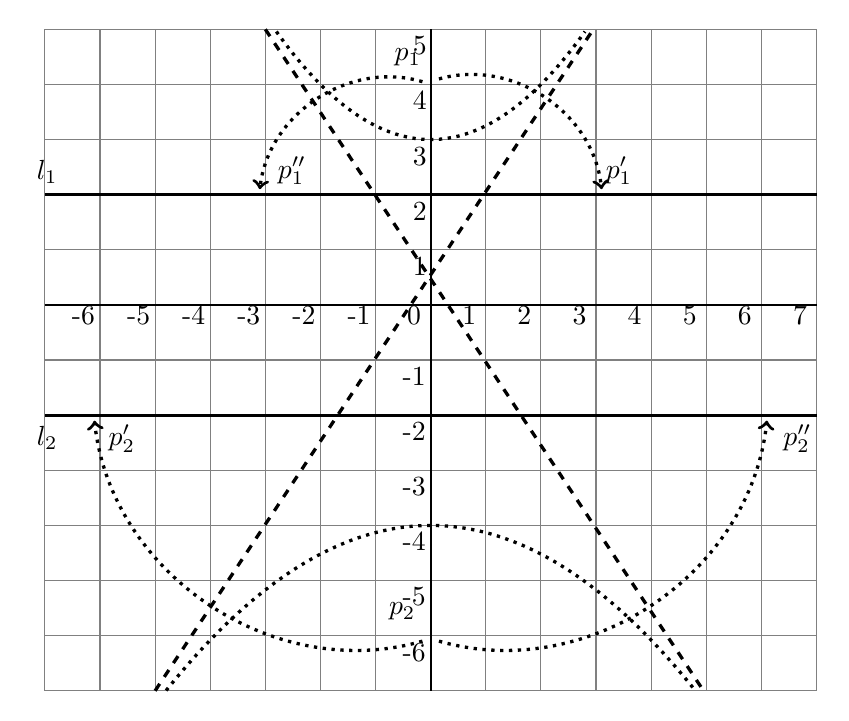
\begin{tikzpicture}[scale=.7]
\draw[step=10mm,white!50!black,thin] (-7,-7) grid (7,5);
\draw[thick] (-7,0) -- (7,0);
\draw[thick] (0,-7) -- (0,5);
\foreach \x in {-6,...,7}
  \node at (\x-.3,-.2) {\sm{\x}};
\foreach \y in {1,...,5}
  \node at (-.2,\y-.3) {\sm{\y}};
\foreach \y in {-6,...,-1}
  \node at (-.3,\y-.3) {\sm{\y}};
  
\coordinate (P1) at (0,4);
\coordinate (P2) at (0,-6);
\coordinate (P1P) at (3.1,2);
\coordinate (P2P) at (-6.12,-2);
\coordinate (P1PP) at (-3.1,2);
\coordinate (P2PP) at (6.12,-2);

\vertex{P1};
\vertex{P2};
\vertex{P1P};
\vertex{P2P};
\vertex{P1PP};
\vertex{P2PP};

\node[above left,yshift=3pt] at (P1) {$p_1$};
\node[above left,xshift=-2pt,yshift=2pt] at (P2) {$p_2$};
\node[above right,xshift=-2pt] at (P1P) {$p_1'$};
\node[below right,xshift=2pt] at (P2P) {$p_2'$};
\node[above right,xshift=3pt] at (P1PP) {$p_1''$};
\node[below right,xshift=2pt] at (P2PP) {$p_2''$};

\draw[very thick] (-7,2) -- node[very near start,above,xshift=-34pt] {$l_1$} (7,2);
\draw[very thick] (-7,-2) -- node[very near start,below,xshift=-34pt] {$l_2$} (7,-2);

\draw[domain=-4.8:4.8,samples=50,very thick,dotted] plot (\x,{-.13*\x*\x-4});
\draw[domain=-2.8:2.8,samples=50,very thick,dotted] plot (\x,{.25*\x*\x+3});

\draw[very thick,dashed] (-5,-7) -- (2.95,5);
\draw[very thick,dashed] (-3,5) -- (4.95,-7);

\draw[very thick,dotted,->,bend left=50] (.15,4.1) to (3.1,2.1);
\draw[very thick,dotted,->,bend right=50] (-.15,4.05) to (-3.1,2.1);

\draw[very thick,dotted,->,bend right=50] (.15,-6.1) to (6.1,-2.1);
\draw[very thick,dotted,->,bend left=50] (-.15,-6.1) to (-6.1,-2.1);

\end{tikzpicture}
%\includegraphics[width=0.9\textwidth]{Fig10_7}
\caption{Axiome  $6$.}\label{f.origami-axiom6}
\end{figure}

Pour qu'un pli place simultanément $p_1$ sur $l_1$ et $p_2$ sur $l_2$, il faut que ce soit une tangente commune aux deux paraboles. Il peut y avoir zéro, un, deux ou trois tangentes communes  (fig.~\ref{f.two-para-1-zero}, \ref{f.two-para-1-one}, \ref{f.two-para-1-two}, \ref{f.two-para-1-three}).

\vspace{0.4cm}

\begin{minipage}{0.4\textwidth}
\centering   
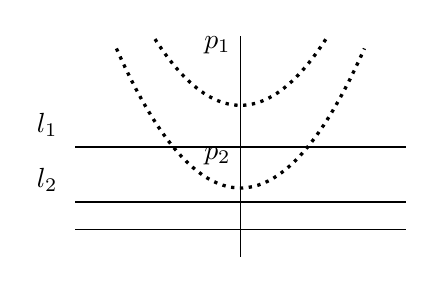
\begin{tikzpicture}[scale=.35]
\draw (-6,0) -- (6,0);
\draw (0,-1) -- (0,7);
\coordinate (P1) at (0,6);
\coordinate (P2) at (0,2);
\vertex{P1};
\vertex{P2};
\node[above left] at (P1) {$p_1$};
\node[above left] at (P2) {$p_2$};
\draw[thick] (-6,3) -- node[very near start,above,xshift=-25pt] {$l_1$} (6,3);
\draw[thick] (-6,1) -- node[very near start,above,xshift=-25pt] {$l_2$} (6,1);
\draw[domain=-3.1:3.1,samples=50,very thick,dotted] plot (\x,{.25*\x*\x+4.5});
\draw[domain=-4.5:4.5,samples=50,very thick,dotted] plot (\x,{.25*\x*\x+1.5});
\end{tikzpicture}
%\includegraphics[width=\textwidth]{Fig10_8a}
         \captionof{figure}{Pas de tangente commune.}\label{f.two-para-1-zero}
         
     \end{minipage}
     \hspace{3em}
     \begin{minipage}{0.4\textwidth}
\centering      
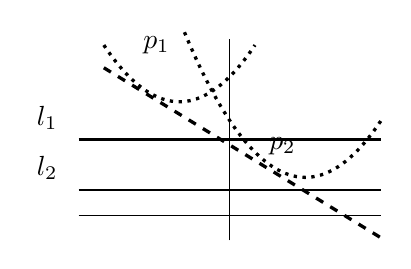
\begin{tikzpicture}[scale=.32]
\draw (-6,0) -- (6,0);
\draw (0,-1) -- (0,7);
\coordinate (P1) at (-2,6);
\coordinate (P2) at (3,2);
\vertex{P1};
\vertex{P2};
\node[above left] at (P1) {$p_1$};
\node[above left] at (P2) {$p_2$};
\draw[thick] (-6,3) -- node[very near start,above,xshift=-25pt] {$l_1$} (6,3);
\draw[thick] (-6,1) -- node[very near start,above,xshift=-25pt] {$l_2$} (6,1);
\draw[domain=-5:1,samples=50,very thick,dotted] plot (\x,{.25*(\x+2)*(\x+2)+4.5});
\draw[domain=-1.8:6,samples=50,very thick,dotted] plot (\x,{.25*(\x-3)*(\x-3)+1.5});
\draw[very thick,dashed] (-5,5.85) -- (6,-.9);
\end{tikzpicture}
%\includegraphics[width=\textwidth]{Fig10_8b}
         \captionof{figure}{Une tangente commune.}\label{f.two-para-1-one}
     \end{minipage}

\vspace{0.4cm}


\begin{minipage}{0.42\textwidth}
\centering   
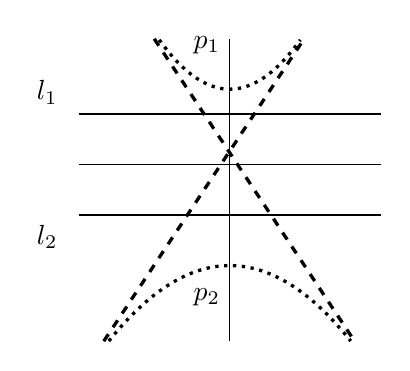
\begin{tikzpicture}[scale=.32]
\draw (-6,0) -- (6,0);
\draw (0,-7) -- (0,5);
\coordinate (P1) at (0,4);
\coordinate (P2) at (0,-6);
\vertex{P1};
\vertex{P2};
\node[above left] at (P1) {$p_1$};
\node[above left] at (P2) {$p_2$};
\draw[thick] (-6,2) -- node[very near start,above,xshift=-25pt] {$l_1$} (6,2);
\draw[thick] (-6,-2) -- node[very near start,below,xshift=-25pt] {$l_2$} (6,-2);
\draw[domain=-4.8:4.8,samples=50,very thick,dotted] plot (\x,{-.13*\x*\x-4});
\draw[domain=-2.8:2.8,samples=50,very thick,dotted] plot (\x,{.25*\x*\x+3});
\draw[very thick,dashed] (-5,-7) -- (2.95,5);
\draw[very thick,dashed] (-3,5) -- (4.95,-7);
\end{tikzpicture}
%\includegraphics[width=\textwidth]{Fig10_9a}
         \captionof{figure}{Deux tangentes communes.}\label{f.two-para-1-two}
         
     \end{minipage}
     \hspace{3em}
     \begin{minipage}{0.42\textwidth}
\centering     
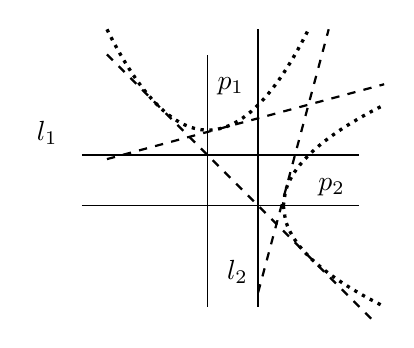
\begin{tikzpicture}[scale=.32]
\draw (-5,0) -- (6,0);
\draw (0,-4) -- (0,6);
\coordinate (P1) at (0,4);
\coordinate (P2) at (4,0);
\vertex{P1};
\vertex{P2};
\node[above right] at (P1) {$p_1$};
\node[above right] at (P2) {$p_2$};
\draw[thick] (-5,2) -- node[very near start,above,xshift=-25pt] {$l_1$} (6,2);
\draw[thick] (2,-4) -- node[very near start,left] {$l_2$} (2,7);
\draw[domain=-4:4,samples=50,very thick,dotted] plot (\x,{.25*\x*\x+3});
\draw[domain=3:7,samples=50,very thick,dotted] plot (\x,{sqrt(4*\x-12)});
\draw[domain=3:7,samples=50,very thick,dotted] plot (\x,{-sqrt(4*\x-12)});

\draw[thick,dashed,domain=-4:6.5] plot (\x,-\x+2);
\draw[thick,dashed,domain=-4:7] plot (\x,.27*\x+2.93);
\draw[thick,dashed,domain=2:4.8] plot (\x,3.73*\x-10.9);
\end{tikzpicture}
%\includegraphics[width=\textwidth]{Fig10_9b}
         \captionof{figure}{Trois tangentes communes.}\label{f.two-para-1-three}
     \end{minipage}

\vspace{0.4cm}


L'équation d'une parabole arbitraire est assez complexe, nous limitons donc la présentation aux paraboles dont l'axe de symétrie est l'axe $x$ ou $y$.

\subsection{Détermination de l'équation d'un pli}

Soit $(0,f)$ le foyer d'une parabole dont la droite directrice est $y=d$. Soit $p=f-d$, la distance algébrique  entre le foyer et la directrice.\footnote{Nous avons utilisé la notation $p_i$ pour les points ; l'utilisation de $p$ ici peut prêter à confusion mais c'est la notation standard. On appelle $p$  le paramètre de la parabole.} Si le sommet de la parabole est sur l'axe $x$, l'équation de la parabole est $y=x^2/(2p)$. Pour déplacer la parabole vers le haut ou vers le bas de l'axe des $y$ de sorte que son sommet soit en $(0,h)$, ajoutons $h$ à l'équation de la parabole (fig.~\ref{f.elements-parabola}):
\[y=\frac{x^2}{2p}+h\,.\]

%\begin{figure}[htb]
%\centering
%\includegraphics[width=0.9\textwidth]{Fig10_10}
%\caption{Les éléments de définition d'une parabole.}\label{f.elements-parabola}
%\end{figure}

\begin{figure}[htb]
\begin{center}
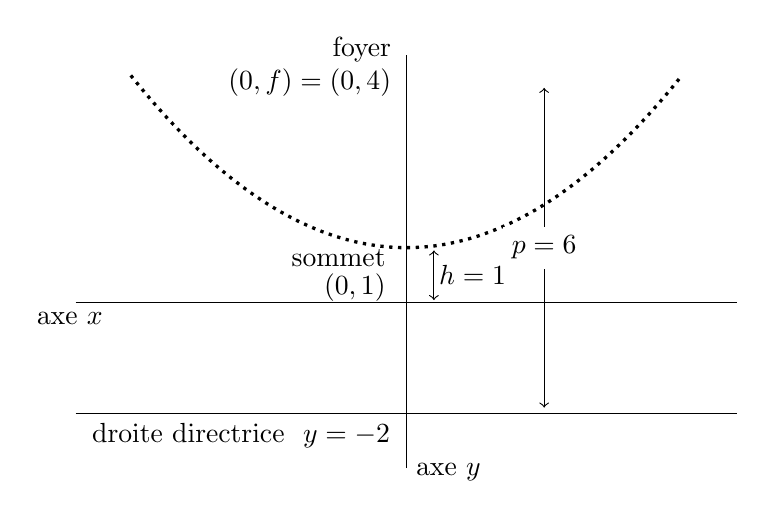
\begin{tikzpicture}[scale=.7]
\draw (-6,0) -- node[very near start,below,xshift=-32pt] {\textrm{axe} $x$}(6,0);
\draw (0,-3) -- node[very near start,right,yshift=-20pt] {\textrm{axe} $y$}(0,4.5);
\draw (-6,-2) -- node[near start,below] {\textrm{droite directrice} $\ y=-2$} (6,-2);
\draw[domain=-5:5,samples=50,very thick,dotted] plot (\x,{\x*\x/8+1});
\coordinate (F) at (0,4);
\coordinate (V) at (0,1);
\coordinate (Y) at (0,-2);
\vertex{F};
\node[left,xshift=-2pt,yshift=0pt] at (F) {$(0,f)=(0,4)$}; \node[above left,xshift=-2pt,yshift=4pt] at (F) {\textrm{foyer}};
\node[below left,xshift=-4,yshift=3pt] at (V) {\textrm{sommet}};
\node[below left,xshift=-4,yshift=-6pt] at (V) {$(0,1)$};
\draw[<->] (2.5,-1.9) -- node[fill=white] {$p=6$} +(0,5.8);
\draw[<->] (.5,.05) -- +(0,.9);
\node at (1.2,.5) {$h=1$} +(0,.9);
\end{tikzpicture}
\end{center}
\caption{Les éléments de définition d'une parabole.}\label{f.elements-parabola}
\end{figure}

Posons $a=2ph$ de sorte que l'équation de la parabole soit 
\begin{subequations}
\begin{align}
y&=\frac{x^2}{2p}+\frac{a}{2p}\,,\\
x^2-2py+a&=0\,.\label{eq.eq-parabola}
\end{align}
\end{subequations}
L'équation de la parabole de la figure \ref{f.elements-parabola} est  $x^2-12y +12=0$.

Substituons l'équation d'une droite arbitraire $y=mx+b$ dans l'équation~\ref{eq.eq-parabola} pour obtenir une équation pour les points d'intersection de la droite et de la parabole :
\begin{align*}
x^2-2p(mx+b)+a&=0\,,\\
x^2+(-2mp)x+(-2pb+a)&=0\,.
\end{align*}
La droite sera tangente à la parabole si et seulement si cette équation du second degré a exactement une solution, c'est-à-dire si et seulement si son discriminant est nul :
\begin{subequations}
\begin{align}
(-2mp)^2\:-\:4\cdot 1\cdot (-2pb+a)&=0\,,\\
m^2p^2+2pb-a&=0\,.\slabel{eq.disc}
\end{align}
\end{subequations}

Il s'agit d'une équation avec des variables $m$ et $b$ pour les tangentes à la parabole. Pour obtenir les tangentes communes aux deux paraboles, nous devons résoudre simultanément les équations pour les deux paraboles.



\begin{example}\mbox{}

\noindent\textbf{Parabole 1:} foyer $(0,4)$, droite directrice $y=2$, sommet $(0,3)$.

\noindent{}$p=2$, $a=2\cdot 2\cdot 3=12$. L'équation de cette parabole est 
\[
x^2-4y +12=0\,.
\]
En substituant $p$ et $a$ dans l'équation~\ref{eq.disc} et en simplifiant, on obtient 
\[
m^2+b-3=0\,.
\]

\noindent\textbf{Parabole 2:} foyer $(0,-4)$, droite directrice $y=-2$, sommet $(0,-3)$.

\noindent{}$p=-2$, $a=2\cdot -2\cdot -3=12$. L'équation de la parabole est 
\[
x^2+4y+12=0\,.
\]
En substituant $p$ et $a$ dans l'équation~\ref{eq.disc} et en simplifiant, on obtient 
\[
m^2-b-3=0\,.
\]
Les solutions des deux équations 
\begin{align*}
m^2+b-3&=0\,,\\
m^2-b-3&=0
\end{align*}
sont $m=\pm\sqrt{3}\approx \pm \mbox{1,73}$ et $b=0$. Il existe deux tangentes communes :
\[
y=\sqrt{3}x\,,\quad y=-\sqrt{3}x\,.
\]
\end{example}

\begin{example}\mbox{}

\noindent\textbf{Parabole 1:}
inchangée.

\noindent\textbf{Parabole 2:} foyer $(0,-6)$, droite directrice $y=-2$, sommet $(0,-4)$.

\noindent{}$p=-4$, $a=2\cdot -4\cdot -4=32$. L'équation de la parabole est 
\[
x^2+8y +32=0\,.
\]
En substituant $p$ et $a$ dans l'équation~\ref{eq.disc} et en simplifiant, on obtient 
\[
2m^2-b-4=0\,.
\]
Les solutions des deux équations 
\begin{align*}
m^2+b-3&=0\,,\\
2m^2-b-4&=0
\end{align*}
sont $m=\pm\sqrt{\displaystyle\frac{7}{3}}\approx \pm \mbox{1,53}$ et $b=\displaystyle\frac{2}{3}$. Il y a deux tangentes communes :
\[
y=\sqrt{\frac{7}{3}}x+\frac{2}{3}\,,\quad y=-\sqrt{\frac{7}{3}}x+\frac{2}{3}\,.
\]
\end{example}

%%%%%%%%%%%%%%%%%%%%%%%%%%%%%%%%%%%%%%%%%%%%%%%%%%%%%%%%%%%%%%%%

\begin{example}\mbox{}

\noindent Définissons maintenant une parabole dont l'axe de symétrie est l'axe $x$.

\noindent\textbf{Parabole 1:} inchangée.

\noindent\textbf{Parabole 2:} foyer $(4,0)$, droite directrice $x=2$, sommet $(3,0)$.

\noindent{}$p=2$, $a=2\cdot 2\cdot 3=12$. L'équation de la parabole est 
\begin{align}
y^2-4x+12 = 0\,.\label{eq.x-symmetry-parabola}
\end{align}
C'est une équation avec $x$ et $y^2$ au lieu de $x^2$ et $y$, donc l'équation~\ref{eq.disc} ne peut pas être utilisée et nous devons refaire les calculs.

Substituons l'équation d'une droite dans l'équation~\ref{eq.x-symmetry-parabola} :
\begin{align*}
(mx+b)^2-4x+12&=0\,,\\
m^2x^2+(2mb-4)x+(b^2+12)&=0\,.
\end{align*}
\'Ecrivons que le discriminant est égal à zéro et simplifions :
\begin{align*}
(2mb-4)^2\:-\:4m^2(b^2+12)&=0\,,\\
-3m^2-mb+1&=0\,.
\end{align*}
Si on essaie de résoudre les deux équations 
\begin{align*}
m^2+b-3&=0\,,\\
-3m^2-mb+1&=0\,,
\end{align*}
on obtient une équation de degré trois en la variable $m$ :
\begin{align}
m^3-3m^2-3m+1=0\,.\label{eq.cubic}
\end{align}
Comme une équation de degré trois a au moins une et au plus trois solutions réelles, il peut y avoir une, deux ou trois tangentes communes.

La formule pour résoudre les équations générales de degré trois  est assez compliquée. On a donc utilisé une calculatrice sur internet et obtenu les trois solutions :
\[m=\approx{3,73},\:m=-1,\:m\approx\mbox{0,27}\,.\]
D'après la forme de l'équation~\ref{eq.cubic}, on peut deviner que $m=1$ ou $m=-1$ est une solution :
\begin{align*}
1^3-3\cdot 1^2-3\cdot 1+1&=-4\,,\\
(-1)^3-3\cdot (-1)^2-3\cdot(-1)+1&=0\,.
\end{align*}
Divisons l'équation~\ref{eq.cubic} par $m-(-1)=m+1$ pour obtenir l'équation du second degré $m^2-4m+1$,  dont les racines sont les deux autres solutions de l'équation du troisième degré:  $m=2\pm\sqrt{3}\approx \mbox{3,73}; \mbox{0,27}$.
\end{example}

%%%%%%%%%%%%%%%%%%%%%%%%%%%%%%%%%%%%%%%%%%%%%%%%%%%%%%%%%%%%%%%%

\subsection{Détermination des équations des réflexions}
On cherche la position du symétrique  $p_1'=(x_1',y_1')$ de $p_1=(x_1,y_1)$ par rapport à une droite tangente $l_t$ dont l'équation est $y=m_tx+b_t$. On commence par trouver la droite $l_p$ d'équation $y=m_px+b_p$ qui est perpendiculaire à $l_t$ et passe par $p_1$ :
\begin{align*}
y&=-\frac{1}{m_t}x+b_p\,,\\
y_1&=-\frac{1}{m_t}x_1+b_p\,,\\
y&=\frac{-x}{m_t}+\left(y_1+\frac{x_1}{m_t}\right)\,.
\end{align*}
Trouvons ensuite l'intersection $p_t=(x_t,y_t)$ de $l_t$ et $l_p$ :
%
\begin{align*}
m_tx_t+b_t&=\frac{-x_t}{m_t}+\left(y_1+\frac{x_1}{m_t}\right)\,,\\
x_t&=\frac{\left(y_1+\displaystyle\frac{x_1}{m_t}-b_t\right)}{\left(m_t+\displaystyle\frac{1}{m_t}\right)}\,,\\
y_t&=m_tx_t+b_t\,.
\end{align*}
$p_t$ est le milieu de  $p_1$ et $p_1'$ :
\begin{align*}
x_t&=\displaystyle\frac{x_1+x_1'}{2}\,,\quad  x_1'=2x_t-x_1\,,\\
y_t&=\displaystyle\frac{y_1+y_1'}{2}\,,\quad  y_1'=2y_t-y_1\,.
\end{align*}



\begin{example}
Soit $l_t$ d'équation $y=\sqrt{3}x+0$ et soit $p_1=(0,4)$ :
\begin{align*}
x_t&=\frac{\left(4+\displaystyle\frac{0}{\sqrt{3}}-0\right)}{\left(\sqrt{3}+\displaystyle\frac{1}{\sqrt{3}}\right)}=\sqrt{3}\,,\\
y_t&=\sqrt{3}\sqrt{3}+0=3\,,\\
x_1'&=2x_t-x_1=2\sqrt{3}\approx \mbox{3,46}\,,\\
y_1'&=2y_t-y_1= 2\,.
\end{align*}
\end{example}

%%%%%%%%%%%%%%%%%%%%%%%%%%%%%%%%%%%%%%%%%%%%%%%%%%%%%%%%%%%%%%%%

\subsection{Tangentes à une parabole}\label{s.parabola}

Nous souhaitons démontrer que les plis de l'axiome~$6$ sont tangents aux paraboles.
La figure~\ref{f.parabola-locus} montre cinq points
$p_i$, $i=1,\ldots,5$, chaque point $p_i$ étant à une distance $a_i$ du foyer et de la droite directrice. Traçons  des droites perpendiculaires à la droite directrice passant par $p_i$ et désignons par $p_i'$ les intersections de ces droites avec la droite directrice. D'après l'axiome~$2$, il existe des plis $l_i$ passant par $p_i$ qui placent $p$ sur la droite directrice. Les points $p_i'$ sont les symétriques de $p$ par rapport aux plis. La figure \ref{f.parabola-locus} montre le pli $l_1$ passant par $p_1$ et le point  $p_1'$.

\begin{figure}[ht]
\centering
\begin{tikzpicture}[scale=.8]
\draw (-6,0) -- node[very near start,below,xshift=-32pt] {axe $x$} (6,0);
\draw (0,-3) -- node[very near start,right,yshift=-15pt] {axe $y$} (0,4.5);
\draw[thick] (-6,-2) -- node[near end,below] {directrice $\quad y=-f$} (6,-2);
\draw[domain=-6:6,samples=50,very thick,dotted] plot (\x,{\x*\x/8});
\coordinate (F) at (0,2);
\vertex{F};
\node[above left,xshift=-2pt,yshift=15pt] at (F) {$(0,f)$};
\node[above left,xshift=-5pt,yshift=26pt] at (F) {foyer}; \node[above right] at (F) {$p$};
\coordinate (vertex) at (0,0);
\vertex{vertex};
\node[below right] at (vertex) {$p_2$};
\coordinate (FP) at (-5,-2);
\node[below] at (FP) {$p_1'$};
\coordinate (F1) at (2,.5);
\vertex{F1};
\node[below right] at (F1) {$p_3$};
\coordinate (F2) at (3,1.125);
\vertex{F2};
\node[below right] at (F2) {$p_4$};
\coordinate (F3) at (5,3.125);
\vertex{F3};
\node[below right] at (F3) {$p_5$};
\coordinate (F4) at (-5,3.125);
\vertex{F4};
\node[above right] at (F4) {$p_1$};
\draw (F) -- node[left] {$a_2$} (0,0) -- node[left] {$a_2$} (0,-2);
\draw (F) -- node[near end,left] {$a_3$} (F1) -- node[left] {$a_3$} (2,-2);
\draw (F) -- node[near end,above] {$a_4$} (F2) -- node[left] {$a_4$} (3,-2);
\draw (F) -- node[above] {$a_5$} (F3) -- node[left] {$a_5$} (5,-2);
\draw (F) -- node[above] {$a_1$} (F4) -- node[left] {$a_1$} (FP);
\draw[very thick,dashed] ($(F4)!-.4!(-2.5,0)$) -- node[near end,right,xshift=2pt] {$l_1$} ($(F4)!1.8!(-2.5,0)$);
\draw (0,-2) rectangle +(9pt,9pt);
\draw (2,-2) rectangle +(9pt,9pt);
\draw (3,-2) rectangle +(9pt,9pt);
\draw (5,-2) rectangle +(9pt,9pt);
\draw (-5,-2) rectangle +(9pt,9pt);
\end{tikzpicture}
%\includegraphics[width=\textwidth]{Fig10_11}
\caption{La tangente comme lieu géométrique.}\label{f.parabola-locus}
\end{figure}



\begin{figure}[htbp]
\centering
\begin{tikzpicture}[scale=.8]
\draw[thick] (-6,-2) -- node[near end, below] {$d$} (6,-2);
\draw[domain=-5.5:5.5,samples=50,very thick,dotted] plot (\x,{\x*\x/8});
\coordinate (F) at (0,2);
\vertex{F};
\node[above right] at (F) {$p$};
\coordinate (FP) at (-3,-2);
\node[below] at (FP) {$p'$};
\coordinate (F4) at (-3,1.125);
\vertex{F4};
\node[above right] at (F4) {$r$};
\coordinate (F5) at (-5,2.775);
\vertex{F5};
\node[left,yshift=-4pt] at (F5) {$q$};
\coordinate (F5p) at (-5,-2);
\node[below] at (F5p) {$p''$};
\draw (F) -- node[above] {$$} (F4) -- node[left] {$$} (FP);
\draw (F) -- node[above] {$$} (F5);
\draw (F5) -- node[left] {$$} (F5p);
\draw[thick,dashed,name path=fold] ($(F4)+(140:4)$) -- (F4) -- node[below,xshift=3pt,yshift=-4pt] {$l$} ($(F4)+(-40:5.3)$);
\draw (FP) rectangle +(10pt,10pt);
\draw (F5p) rectangle +(10pt,10pt);
\draw (F5) -- (FP);
\draw[name path=base] (F) -- (FP);
\path [name intersections = {of = base and fold, by = {G}}];
\node[below,yshift=-4pt] at (G) {$s$};
\draw[rotate=140] (G) rectangle +(10pt,10pt);
\path (FP) -- node[left] {$$} (F5);
\path (F) -- node[below] {$$} (G) -- node[below] {$$} (FP);
\end{tikzpicture}
%\includegraphics[width=\textwidth]{Fig10_12}

\caption{La démonstration que le pli est une tangente à la parabole.}\label{f.tangent-proof}
\end{figure}

\begin{theorem}\label{thm.parabola-tangents}
Les plis de l'axiome~$6$ sont les tangentes aux deux paraboles qui sont les lieux des points équidistants de $p_1$ et $l_1$ (respectivement $p_2$ et $l_2$).
\end{theorem}
\begin{proof}
Dans la figure~\ref{f.tangent-proof}, le foyer est $p$ et la droite directrice est $d$. Le point $p'$ est  sur la droite directrice et $l$ est le pli qui envoie $p$ sur $p'$. Soit $s$ l'intersection de $\overline{pp'}$ et $l$. Alors $\overline{ps}=\overline{p's}$ et $l\perp \overline{pp'}$ puisque $l$ est la médiatrice de $\overline{pp'}$.

Soit $r$ l'intersection de la droite perpendiculaire à $d$ passant par $p'$ et du pli $l$. Alors $\triangle psr\cong \triangle p'sr$ (deux côtés et un angle identiques). Il s'ensuit que 
$\overline{pr}=\overline{p'r}$ donc $r$ est un point de la parabole. 

Supposons que le pli $l$ recoupe la parabole en un point $q\neq r$. Soit $p''$ la projection orthogonale de $q$ sur la droite directrice $d$. On a $p''\neq p'$. Puisque $q$ est sur la parabole, on a $\overline{pq}=\overline{p''q}$. Puisque $q$ est sur le pli $l$ qui est la médiatrice de $\overline{pp'}$, on a $\overline{pq}=\overline{p'q}$. D'où $\overline{p''q}=\overline{p'q}$, ce qui est impossible car $\overline{p'q}$ est l'hypoténuse du triangle rectangle $\triangle qp''p'$:  l'hypoténuse ne peut être  égale à l'un des autres côtés du triangle rectangle. Par conséquent, le pli $l$ n'a qu'une seule intersection avec la parabole et doit être une tangente.
%Choisissons un point $p''$ sur la droite directrice qui est distinct de $p'$ et supposons que le pli $l$ envoie aussi $p$ sur $p''$. Soit $q$ l'intersection de la perpendiculaire à $d$ passant par $p''$ et du pli $l$. $\triangle psq\cong \triangle p'sq$ donc $\overline{pq}=\overline{p'q}=c$. Posons $\overline{qp''}=e$. Si $q$ est un point de la parabole, alors $e=\overline{qp''}=\overline{qp}=c$, mais $c$ est l'hypoténuse du triangle rectangle $\triangle qp''p'$ et il n'est pas possible que l'hypoténuse soit égale à l'un des autres côtés du triangle rectangle. Par conséquent, le pli $l$ n'a qu'une seule intersection avec la parabole et doit être une tangente.
\end{proof}

%%%%%%%%%%%%%%%%%%%%%%%%%%%%%%%%%%%%%%%%%%%%%%%%%%%%%%%%%%%%%%%%

%\vspace{-4ex}

\section{Axiome 7}\label{s.ax7}


\begin{axiom}
Étant donné un point $p_1$ et deux droites $l_1$ et $l_2$, il existe un pli $l$ qui envoie $p_1$ sur $l_1$ et qui est perpendiculaire à $l_2$ (fig.~\ref{f.origami-axiom7}).
\end{axiom}

Le pli est le lieu géométrique de tous les points de la droite perpendiculaire à $l_2$,  équidistants de $p_1$ et $p_1'$, l'image  de $p_1$ sur $l_1$.

\smallskip

\noindent\textbf{Détermination de l'équation du pli.}
Soit $p_1=(x_1,y_1)$. Soient $l_1$ d'équation $y = m_1x + b_1$ et $l_2$ d'équation $y=m_2x+b_2$. Soit $l_p$ la droite contenant $\overline{p_1p_1'}$. Puisque $l\perp l_2$ et $l_p\perp l$, il s'ensuit que $l_p\parallel l_2$ et l'équation de $l_p$ est $y=m_2x+b_p$.

\begin{figure}[tbh]
\centering
\begin{tikzpicture}[scale=.8]
\draw[step=10mm,white!50!black,thin] (-1,-1) grid (9,8);
\draw[thick] (-1,0) -- (9,0);
\draw[thick] (0,-1) -- (0,8);
\foreach \x in {0,...,9}
  \node at (\x-.2,-.2) {\sm{\x}};
\foreach \y in {1,...,8}
  \node at (-.2,\y-.3) {\sm{\y}};
  
\coordinate (P1) at (5,3);
\node[below left] at (P1) {$p_1$};
\vertex{P1};

\coordinate (P1P) at (2.75,5.25);
\node[left,xshift=-4pt] at (P1P) {$p_1'$};
\vertex{P1P};

\draw (1,0) -- node[very near start,right,xshift=2pt] {$l_1$} (3,6);
\draw[name path=l2] (8,3) -- node[very near start,right,xshift=-2pt,yshift=6pt] {$l_2$} (5,6);

\draw ($(1,0)!-.16!(3,6)$) -- ($(1,0)!1.33!(3,6)$);

\draw ($(8,3)!-.33!(5,6)$) -- ($(8,3)!1.66!(5,6)$);

\draw ($(P1)!-.4!(P1P)$) -- node[very near start,below,yshift=-4pt] {$l_p$} ($(P1)!1.5!(P1P)$);

\draw[very thick,dashed,name path=fold] (-1,-.75) -- node[very near end,above,xshift=4pt,yshift=6pt] {$l$} (7.75,8);

\coordinate (mid) at ($(P1)!.5!(P1P)$);
\node[below,yshift=-8pt] at (mid) {$p_m$};

\path [name intersections = {of = fold and l2, by = {perp}}];
\draw[rotate=-45] (mid) rectangle +(8pt,8pt);
\draw[rotate=-45] (perp) rectangle +(8pt,8pt);


\draw[very thick,dotted,->,bend right=50] (5.05,3.1) to (2.85,5.24);
\end{tikzpicture}
%\includegraphics[width=\textwidth]{Fig10_13}
\caption{Axiome  $7$.}\label{f.origami-axiom7}
\end{figure}

La droite $l_p$ passe par $p_1$, donc $y_1=m_2x_1+b_p$ et son équation est $y=m_2x+(y_1-m_2x_1)$. L'image $p_1'=(x_1',y_1')$ est l'intersection de $l_1$ et $l_p$ :
\begin{align*}
m_1x_1'+b_1&=m_2x_1'+(y_1-m_2x_1)\,,\\
x_1'&=\frac{y_1-m_2x_1-b_1}{m_1-m_2}\,,\\
y_1'&=m_1x_1'+b_1\,.
\end{align*}
Les coordonnées du milieu $p_m=(x_m,y_m)$ sur $l_p$ est 
\[
(x_m,y_m)=\left(\frac{x_1+x_1'}{2},\frac{y_1+y_1'}{2}\right)\,.
\]
$l\perp l_2$ et  $l$ passe par $p_m$. Donc son équation est 
\[
y=-\frac{1}{m_2}x+b_m,
\]
où $b_m$ peut être calculé avec   $y_m=-\displaystyle\frac{1}{m_2}x_m+b_m$:
\[b_m=y_m+\frac{x_m}{m_2}\,.\]
L'équation du pli $l$ est donc 
\[
y=-\frac{1}{m_2}x+\left(y_m+\displaystyle\frac{x_m}{m_2}\right)\,.
\]
\begin{example}
Soit $p_1=(5,3)$. Soient  $l_1$ d'équation $y=3x-3$ et  $l_2$ d'équation $y=-x+11$. Alors 
\begin{align*}
x_1'&=\frac{3-(-1)\cdot 5-(-3)}{3-(-1)}=\frac{11}{4}\,,\\
y_1'&=3\cdot \frac{11}{4} + (-3)=\frac{21}{4}\,,\\
p_m&=\left(\frac{5+\displaystyle\frac{11}{4}}{2},\frac{3+\displaystyle\frac{21}{4}}{2}\right)=\left(\frac{31}{8},\frac{33}{8}\right)\,.
\end{align*}
L'équation du pli $l$ est 
\[
y=-\frac{1}{-1}\cdot x+\left(\frac{33}{8}+\frac{\displaystyle\frac{31}{8}}{-1}\right)=x+\frac{1}{4}\,.
\]
\end{example}

\vspace{-2ex}

\subsection*{Quelle est la surprise ?}

L'origami, l'art du pliage du papier, est pratiqué depuis des centaines d'années. Il est donc surprenant que la formalisation mathématique ne remonte qu'au \textsc{xx}$^\text{e}$ siècle. Il est encore plus surprenant qu'il existe une axiomatisation du pliage du papier. Les mathématiques de l'origami sont un excellent moyen d'apprendre la géométrie analytique, les propriétés des paraboles et le concept de lieu géométrique.

\vspace{-2ex}

\subsection*{Sources}

Les axiomes de l'origami sont présentés dans \cite{wiki:hh-axioms}. Lang \cite{lang} donne des descriptions de constructions d'origami. 
\cite[chap.~10]{martin} contient la théorie détaillée des mathématiques de l'origami, notamment la démonstration que deux paraboles peuvent avoir zéro, un, deux ou trois tangentes communes. La démonstration du théorème~\ref{thm.parabola-tangents} m'a été montrée par Oriah Ben-Lulu. J'ai trouvé qu'un logiciel de géométrie comme {Geogebra} est utile pour comprendre la relation entre la géométrie et l'algèbre des axiomes.

Une présentation claire des équations de degré trois se trouve  dans \cite[chap.~1 et 2]{jorg}.
